%==============================================================
%  EE201 -- Circuit Theory I
%  Lecture 1 : Basic Concepts   --   presentation slides
%  M. Mert Ankaralı, METU EEE
%
%  Compile:  ./build.sh      (or: pdflatex EE201_Lecture_1_slides.tex, twice)
%  Same colour code as the handout:
%      charge = purple, current = blue, voltage = orange, power = green
%==============================================================
\documentclass[11pt,aspectratio=169]{beamer}

\usepackage[T1]{fontenc}
\usepackage[utf8]{inputenc}
\usepackage[english]{babel}
\usepackage{lmodern}
\usepackage{amsmath,amssymb}
\usepackage{booktabs}
\usepackage{array}
\usepackage{colortbl}
\usepackage{tikz}
\usepackage[american,siunitx]{circuitikz}
\usetikzlibrary{arrows.meta,positioning,calc,decorations.pathreplacing,decorations.pathmorphing}

%-------------------- plain METU-flavoured theme --------------
\usetheme{default}
\usecolortheme{default}
\useinnertheme{rectangles}
\setbeamertemplate{navigation symbols}{}
\setbeamertemplate{itemize items}[square]
\setbeamerfont{frametitle}{size=\large,series=\bfseries}
\setbeamerfont{title}{size=\LARGE,series=\bfseries}

\definecolor{metured}{RGB}{155,27,48}
\definecolor{metugray}{RGB}{88,89,91}
\definecolor{metulight}{RGB}{243,240,241}
\definecolor{ccur}{RGB}{0,102,170}
\definecolor{cvolt}{RGB}{214,120,0}
\definecolor{cpow}{RGB}{23,128,74}
\definecolor{ccharge}{RGB}{124,60,160}

\setbeamercolor{structure}{fg=metured}
\setbeamercolor{frametitle}{fg=metured,bg=}
\setbeamercolor{title}{fg=metured}
\setbeamercolor{normal text}{fg=black!88}
\setbeamercolor{block title}{fg=white,bg=metured}
\setbeamercolor{block body}{bg=metulight}
\setbeamercolor{alerted text}{fg=metured}

\setbeamertemplate{frametitle}{%
  \vspace{0.55em}%
  \usebeamerfont{frametitle}\usebeamercolor[fg]{frametitle}\insertframetitle\par
  \vspace{-0.2em}{\color{metured}\rule{\textwidth}{1pt}}\par\vspace{-0.2em}}

\setbeamertemplate{footline}{%
  \hbox{\begin{beamercolorbox}[wd=\paperwidth,ht=2.4ex,dp=1.4ex,leftskip=1.2em,rightskip=1.2em]{}%
  \tiny\color{metugray}\coursecode\ \textbar\ Lecture 1: Basic Concepts
  \hfill \insertframenumber/\inserttotalframenumber
  \end{beamercolorbox}}}

%-------------------- macros ----------------------------------
\newcommand{\coursecode}{EE201}
\newcommand{\term}{Fall 2026--2027}
\newcommand{\Icol}[1]{\textcolor{ccur}{#1}}
\newcommand{\Vcol}[1]{\textcolor{cvolt}{#1}}
\newcommand{\Pcol}[1]{\textcolor{cpow}{#1}}
\newcommand{\Qcol}[1]{\textcolor{ccharge}{#1}}
\newcommand{\uni}[1]{\,\mathrm{#1}}
\newcommand{\A}{\uni{A}} \newcommand{\V}{\uni{V}}
\newcommand{\W}{\uni{W}} \newcommand{\J}{\uni{J}}
\newcommand{\Cb}{\uni{C}} \newcommand{\s}{\uni{s}}

\ctikzset{bipoles/length=0.9cm}
\tikzset{
  curarr/.style={-{Stealth[length=2.6mm]}, ccur, very thick},
  blk/.style={draw=metugray, fill=metulight, rounded corners=2pt,
              minimum height=1.25cm, text width=2.45cm, align=center, font=\scriptsize},
  flowarr/.style={-{Stealth[length=3mm]}, metured, very thick},
  thru/.style={-{Stealth[length=2.2mm]}, ccur, very thick},
  acr/.style={{Stealth[length=2mm]}-{Stealth[length=2mm]}, cvolt, very thick},
  pan/.style={draw=gray!35, fill=metulight, rounded corners=3pt,
              minimum width=3.0cm, minimum height=2.3cm},
  pcap/.style={font=\scriptsize\bfseries, text=metured},
}

% helpers for the four-domain across/through figure
\newcommand{\dmacross}[1]{\draw[acr] (0.45,1.45) -- (2.55,1.45);
  \node[cvolt, font=\scriptsize] at (1.5,1.76) {#1};
  \draw[gray!45, dashed] (0.45,0.28) -- (0.45,1.40);
  \draw[gray!45, dashed] (2.55,0.28) -- (2.55,1.40);}
\newcommand{\dmthrough}[1]{\draw[thru] (0.15,0.05) -- (1.0,0.05);
  \node[ccur, font=\scriptsize, anchor=west] at (1.12,0.05) {#1};}
\newcommand{\dmpanel}[1]{\node[font=\small\bfseries, text=metured] at (1.5,2.30) {#1};}

\hypersetup{colorlinks=true,allcolors=metured}

\title{Lecture 1: Basic Concepts}
\subtitle{EE201 -- Circuit Theory I}
\author{M. Mert Ankaralı}
\institute{\small Department of Electrical and Electronics Engineering\\
           Middle East Technical University}
\date{}

%==============================================================
\begin{document}

%--------------------------------------------------------------
\begin{frame}[plain]
  \titlepage
  \begin{center}\small\color{metugray}
    charge \Qcol{$\blacksquare$}\quad current \Icol{$\blacksquare$}\quad
    voltage \Vcol{$\blacksquare$}\quad power \Pcol{$\blacksquare$}\\[2pt]
    {\scriptsize these colours mean the same thing on every slide and in the notes}
  \end{center}
\end{frame}

%==============================================================
\section{Modelling}
%--------------------------------------------------------------
\begin{frame}{Circuit theory is not about wires}
  \vfill
  \begin{center}
  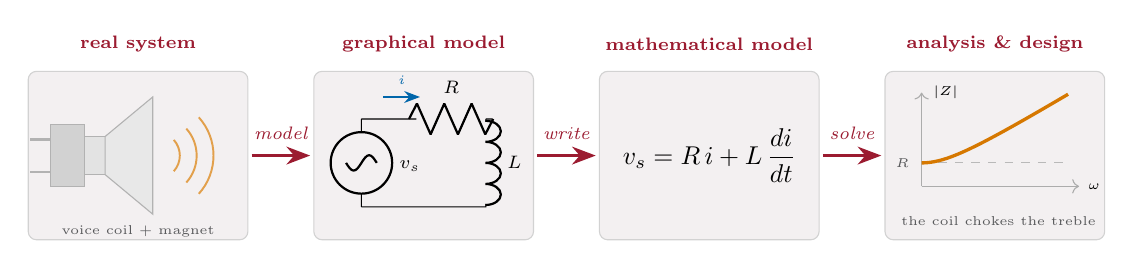
\begin{tikzpicture}[scale=0.93, transform shape]
    \foreach \i/\t in {0/real system, 1/graphical model, 2/mathematical model, 3/analysis \& design}{
      \node[pan] (P\i) at (\i*3.9,0) {};
      \node[pcap] at (\i*3.9,1.52) {\t};
    }
    \foreach \i/\j/\l in {0/1/model, 1/2/write, 2/3/solve}{
      \pgfmathsetmacro\xa{\i*3.9+1.55}\pgfmathsetmacro\xb{\j*3.9-1.55}
      \draw[flowarr] (\xa,0) -- (\xb,0);
      \pgfmathsetmacro\xm{(\i*3.9+\j*3.9)/2}
      \node[font=\scriptsize\itshape, text=metured, above=1pt] at (\xm,0.06) {\l};
    }
    % --- real system: a loudspeaker in cross-section
    \begin{scope}[shift={(-0.15,0)}]
      \fill[gray!35] (-1.05,-0.42) rectangle (-0.58,0.42);
      \draw[gray!60] (-1.05,-0.42) rectangle (-0.58,0.42);
      \fill[gray!22] (-0.58,-0.26) rectangle (-0.30,0.26);
      \draw[gray!60] (-0.58,-0.26) rectangle (-0.30,0.26);
      \fill[gray!18] (-0.30,-0.26) -- (0.35,-0.80) -- (0.35,0.80) -- (-0.30,0.26) -- cycle;
      \draw[gray!60] (-0.30,-0.26) -- (0.35,-0.80) -- (0.35,0.80) -- (-0.30,0.26) -- cycle;
      \draw[gray!60] (0.35,-0.80) -- (0.35,0.80);
      \foreach \r in {0.32,0.55,0.78}{
        \draw[cvolt!70, line width=0.7pt] ([shift=(-42:\r)]0.4,0) arc (-42:42:\r);}
      \draw[gray!60, thick] (-1.05,0.22) -- (-1.32,0.22);
      \draw[gray!60, thick] (-1.05,-0.22) -- (-1.32,-0.22);
      \node[font=\tiny, text=metugray] at (0.15,-1.03) {voice coil + magnet};
    \end{scope}
    % --- graphical model
    \begin{scope}[shift={(3.9,-0.1)}]
      \draw (-0.85,-0.6) to[sV, invert, l_={\scriptsize$v_s$}] (-0.85,0.6);
      \draw (-0.85,0.6) -- (-0.1,0.6) to[R, l=\scriptsize$R$] (0.85,0.6);
      \draw (0.85,0.6) to[L, l=\scriptsize$L$] (0.85,-0.6) -- (-0.85,-0.6);
      \draw[-{Stealth[length=2mm]}, ccur, thick] (-0.55,0.9) -- (-0.05,0.9);
      \node[ccur, font=\tiny] at (-0.3,1.13) {$i$};
    \end{scope}
    % --- mathematical model
    \node at (7.8,0) {$\displaystyle v_s = R\,i + L\,\frac{di}{dt}$};
    % --- analysis
    \begin{scope}[shift={(11.7,-0.42)}]
      \draw[->,gray!65] (-1.0,0) -- (1.15,0) node[right,font=\tiny,black] {$\omega$};
      \draw[->,gray!65] (-1.0,0) -- (-1.0,1.28) node[right=1pt,font=\tiny,black] {$|Z|$};
      \draw[gray!55,dashed] (-1.0,0.32) -- (1.0,0.32);
      \node[font=\tiny, text=metugray, anchor=east] at (-1.05,0.32) {$R$};
      \draw[cvolt, very thick, domain=-1.0:1.0, samples=80, smooth]
           plot (\x, {0.32*sqrt(1+(1.9*(\x+1.0))^2)});
      \node[font=\tiny, text=metugray] at (0.05,-0.48) {the coil chokes the treble};
    \end{scope}
  \end{tikzpicture}
  \end{center}
  \vfill
  \begin{center}
    A real loudspeaker also has a cone, a suspension, a mass, a room around it.\\
    We keep \alert{two numbers}, $R$ and $L$, and throw the rest away.
  \end{center}
  \vfill
  \begin{center}
    {\large\itshape ``All models are wrong, but some are useful.''}\\[3pt]
    {\small\color{metugray} George E. P. Box, 1976}
  \end{center}
\end{frame}

%--------------------------------------------------------------
\begin{frame}{The same pipeline, other domains}
  \vfill
  \begin{center}
  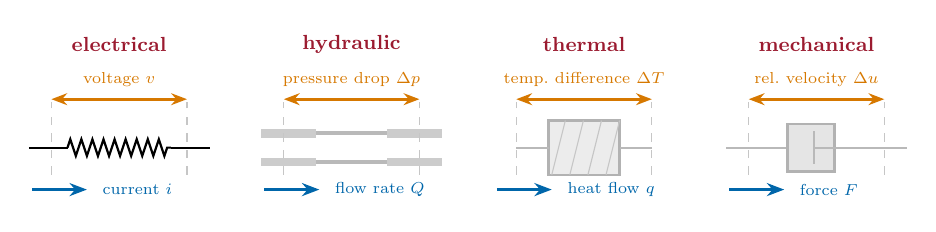
\begin{tikzpicture}[scale=0.82, transform shape]
    % electrical
    \begin{scope}
      \dmpanel{electrical}
      \draw[thick] (0.1,0.7) -- (0.7,0.7);
      \draw[thick, decorate, decoration={zigzag, segment length=4pt, amplitude=3pt}]
            (0.7,0.7) -- (2.3,0.7);
      \draw[thick] (2.3,0.7) -- (2.9,0.7);
      \dmacross{voltage $v$}\dmthrough{current $i$}
    \end{scope}
    % hydraulic
    \begin{scope}[xshift=3.6cm]
      \dmpanel{hydraulic}
      \draw[line width=3pt, gray!40] (0.1,0.92) -- (0.95,0.92);
      \draw[line width=1.4pt, gray!55] (0.95,0.92) -- (2.05,0.92);
      \draw[line width=3pt, gray!40] (2.05,0.92) -- (2.9,0.92);
      \draw[line width=3pt, gray!40] (0.1,0.48) -- (0.95,0.48);
      \draw[line width=1.4pt, gray!55] (0.95,0.48) -- (2.05,0.48);
      \draw[line width=3pt, gray!40] (2.05,0.48) -- (2.9,0.48);
      \dmacross{pressure drop $\Delta p$}\dmthrough{flow rate $Q$}
    \end{scope}
    % thermal
    \begin{scope}[xshift=7.2cm]
      \dmpanel{thermal}
      \fill[gray!15] (0.95,0.28) rectangle (2.05,1.12);
      \draw[gray!60, thick] (0.95,0.28) rectangle (2.05,1.12);
      \foreach \k in {0,1,2,3}{\draw[gray!45] (1.0+\k*0.28,0.28) -- (1.21+\k*0.28,1.12);}
      \draw[thick, gray!55] (0.45,0.7) -- (0.95,0.7);
      \draw[thick, gray!55] (2.05,0.7) -- (2.55,0.7);
      \dmacross{temp.\ difference $\Delta T$}\dmthrough{heat flow $q$}
    \end{scope}
    % mechanical
    \begin{scope}[xshift=10.8cm]
      \dmpanel{mechanical}
      \draw[thick, gray!55] (0.1,0.7) -- (1.05,0.7);
      \draw[thick, gray!55] (1.05,0.33) -- (1.05,1.07);
      \fill[gray!20] (1.05,0.33) rectangle (1.78,1.07);
      \draw[gray!60, thick] (1.05,0.33) rectangle (1.78,1.07);
      \draw[thick, gray!55] (1.46,0.7) -- (2.9,0.7);
      \draw[thick, gray!55] (1.46,0.45) -- (1.46,0.95);
      \dmacross{rel.\ velocity $\Delta u$}\dmthrough{force $F$}
    \end{scope}
  \end{tikzpicture}
  \end{center}
  \vfill
  \begin{columns}[T,onlytextwidth]
    \begin{column}{0.48\textwidth}
      \begin{block}{Across: needs \emph{two} points}
        \small A difference. The second point is usually left unsaid because a reference
        was agreed on long ago --- sea level, atmospheric pressure. A circuit has none,
        so we pick one: \emph{ground}.
      \end{block}
    \end{column}
    \begin{column}{0.48\textwidth}
      \begin{block}{Through: needs \emph{one}}
        \small Measured at a place, with a direction --- and no reference: zero current
        means the same to everyone.
      \end{block}
    \end{column}
  \end{columns}
  \vfill
\end{frame}

%==============================================================
\section{Charge}
%--------------------------------------------------------------
\begin{frame}{\Qcol{Charge}}
  \begin{block}{Definition}
    \textbf{Charge} is the property of matter that makes it feel a force in an
    electromagnetic field. Symbol \Qcol{$q$}, unit \textbf{coulomb (C)}.
  \end{block}
  \vspace{0.3em}
  \begin{columns}[c,onlytextwidth]
    \column{0.52\textwidth}
      \begin{center}
      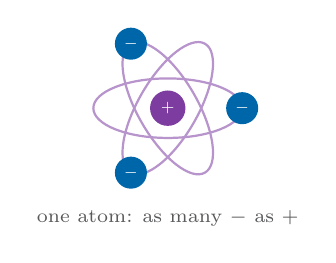
\begin{tikzpicture}[scale=0.9]
        % --- an atom
        \draw[ccharge!55, thick] (0,0) ellipse (1.05 and 0.42);
        \begin{scope}[rotate=60]  \draw[ccharge!55, thick] (0,0) ellipse (1.05 and 0.42); \end{scope}
        \begin{scope}[rotate=-60] \draw[ccharge!55, thick] (0,0) ellipse (1.05 and 0.42); \end{scope}
        \node[circle, fill=ccharge, text=white, inner sep=2.2pt, font=\tiny] at (0,0) {$+$};
        \foreach \p in {(1.05,0), (-0.52,0.91), (-0.52,-0.91)}{
          \node[circle, fill=ccur, text=white, inner sep=1.7pt, font=\tiny] at \p {$-$};}
        \node[font=\scriptsize, text=metugray] at (0,-1.55) {one atom: as many $-$ as $+$};
      \end{tikzpicture}
      \end{center}
    \column{0.44\textwidth}
      \[ e = 1.602\times10^{-19}\Cb \]
      \[ 1\Cb \approx 6.24\times10^{18}\ \text{electron charges} \]
      \vspace{0.2em}
      \begin{itemize}
        \item electron: $-e$ \quad proton: $+e$
        \item \textbf{Charge is conserved} --- never created or destroyed, only moved.
              (This will become KCL.)
      \end{itemize}
  \end{columns}
\end{frame}

%--------------------------------------------------------------
\begin{frame}{A wire is already \alert{full} of charge}
  \begin{columns}[c,onlytextwidth]
    \column{0.46\textwidth}
      \begin{center}
      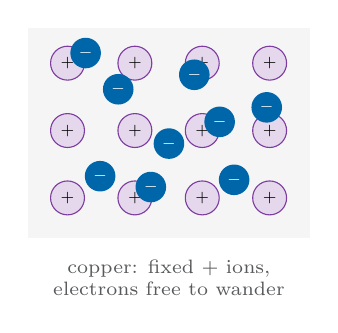
\begin{tikzpicture}[scale=0.92]
        \fill[gray!8] (-0.55,-0.55) rectangle (3.35,2.35);
        \foreach \i in {0,1,2,3}{\foreach \j in {0,1,2}{
          \node[circle, draw=ccharge, fill=ccharge!20, inner sep=2.0pt, font=\tiny]
               at (\i*0.93,\j*0.93) {$+$};}}
        \foreach \p in {(0.45,0.3),(1.4,0.75),(2.3,0.25),(0.7,1.5),(1.75,1.7),
                        (2.75,1.25),(0.25,2.0),(2.1,1.05),(1.15,0.15)}{
          \node[circle, fill=ccur, text=white, inner sep=1.5pt, font=\tiny] at \p {$-$};}
        \node[font=\scriptsize, text=metugray, align=center] at (1.4,-1.1)
             {copper: fixed $+$ ions,\\ electrons free to wander};
      \end{tikzpicture}
      \end{center}
    \column{0.50\textwidth}
      $1\ \mathrm{cm^3}$ of copper contains about
      \[ 8.5\times10^{22}\ \text{free electrons} \;\approx\; \Qcol{13\,600\Cb} \]
      of \emph{mobile} charge --- and its net charge is \alert{zero}.
      \vspace{0.5em}
      \begin{block}{So what is a current?}
        \small Every free electron left a $+$ ion behind. The metal stays neutral;
        current is that charge \emph{drifting}, not charge being poured in.
      \end{block}
  \end{columns}
\end{frame}

%==============================================================
\section{Current}
%--------------------------------------------------------------
\begin{frame}{\Icol{Current}: charge in motion}
  \begin{block}{Definition}
    \[
      \Icol{i(t)} = \frac{dq(t)}{dt}
      \qquad\Longleftrightarrow\qquad
      q(t) = q(t_0) + \int_{t_0}^{t} i(\tau)\,d\tau
    \]
    Unit: \textbf{ampere (A)}, $1\A = 1\Cb/\s$.
  \end{block}
  \vfill
  \begin{center}
  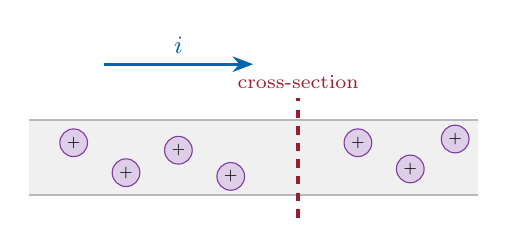
\begin{tikzpicture}[scale=0.95]
    \fill[gray!12] (0,-0.5) rectangle (6,0.5);
    \draw[gray!55, thick] (0,-0.5) -- (6,-0.5);
    \draw[gray!55, thick] (0,0.5) -- (6,0.5);
    \draw[metured, very thick, dashed] (3.6,-0.8) -- (3.6,0.8);
    \node[metured, font=\scriptsize, above] at (3.6,0.8) {cross-section};
    \foreach \x/\y in {0.6/0.2, 1.3/-0.2, 2.0/0.1, 2.7/-0.25, 4.4/0.2, 5.1/-0.15, 5.7/0.25}{
      \node[circle, draw=ccharge, fill=ccharge!25, inner sep=1.2pt, font=\tiny] at (\x,\y) {$+$};}
    \draw[curarr] (1.0,1.25) -- (3.0,1.25) node[midway, above, font=\small] {$\Icol{i}$};
  \end{tikzpicture}
  \end{center}
\end{frame}

%--------------------------------------------------------------
\begin{frame}{The arrow is a \alert{choice}, not a fact}
  \vfill
  \begin{center}
  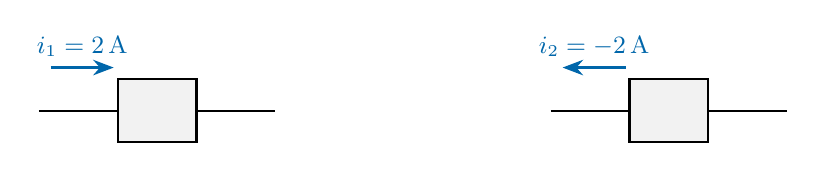
\begin{tikzpicture}
    \begin{scope}
      \draw[thick] (0,0) -- (1,0); \draw[thick] (2,0) -- (3,0);
      \draw[thick, fill=gray!10] (1,-0.4) rectangle (2,0.4);
      \draw[curarr] (0.15,0.55) -- (0.95,0.55) node[midway,above,font=\small]{$\Icol{i_1 = 2\A}$};
    \end{scope}
    \begin{scope}[xshift=6.5cm]
      \draw[thick] (0,0) -- (1,0); \draw[thick] (2,0) -- (3,0);
      \draw[thick, fill=gray!10] (1,-0.4) rectangle (2,0.4);
      \draw[curarr] (0.95,0.55) -- (0.15,0.55) node[midway,above,font=\small]{$\Icol{i_2 = -2\A}$};
    \end{scope}
  \end{tikzpicture}
  \end{center}
  \vfill
  \begin{center}
    \textbf{Same physical situation.} The arrow says which way we call positive;\\
    the sign of the number says which way the charge really goes.
  \end{center}
  \vfill
  {\small A negative answer is not a mistake --- it is the model telling you something.}
\end{frame}

%--------------------------------------------------------------
\begin{frame}{Two numbers worth knowing}
  \begin{columns}[T,onlytextwidth]
    \column{0.47\textwidth}
      \begin{block}{How much is a coulomb?}
        A $4000$ mAh phone battery:
        \[ Q = 4\A \times 3600\s = 14\,400\Cb \]
        \[ \approx 9\times10^{22}\ \text{elementary charges} \]
      \end{block}
      \small
      At $10^{22}$ charges, the lumpiness of charge is invisible. We may treat
      \Qcol{$q(t)$} as a \alert{smooth} quantity --- which is what lets us write
      $dq/dt$ at all.
    \column{0.47\textwidth}
      \begin{block}{How fast do the charges move?}
        $1\A$ in a $1\ \mathrm{mm^2}$ copper wire:
        \begin{center}
          each electron drifts at about\\[3pt]
          \alert{$0.07$ mm/s} $\;\approx\;$ 1 metre in 4 hours
        \end{center}
      \end{block}
      \small
      Yet the lamp lights the instant you flip the switch. The carriers crawl;
      the \emph{signal} that starts them travels near the speed of light.
  \end{columns}
  \vfill
  \begin{center}\small\color{metugray}
    We come back to that gap when we define a \emph{lumped} circuit.
  \end{center}
\end{frame}

%--------------------------------------------------------------
\begin{frame}{Conventional current}
  \vfill
  \begin{center}
  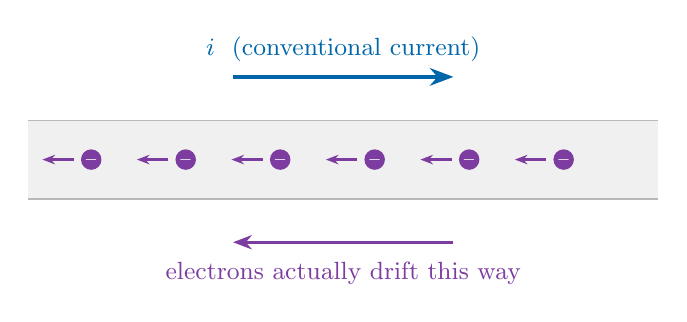
\begin{tikzpicture}[scale=1.0]
    % wire
    \fill[gray!12] (0,0) rectangle (8,1.0);
    \draw[gray!55] (0,0) -- (8,0) (0,1.0) -- (8,1.0);
    % electrons drifting left
    \foreach \x in {0.8,2.0,3.2,4.4,5.6,6.8}{
      \fill[ccharge] (\x,0.5) circle (0.13);
      \node[white, font=\tiny] at (\x,0.5) {$-$};
      \draw[-{Stealth[length=1.6mm]}, ccharge, thick] (\x-0.22,0.5) -- (\x-0.62,0.5);
    }
    % current arrow
    \draw[-{Stealth[length=3mm]}, ccur, very thick] (2.6,1.55) -- (5.4,1.55);
    \node[ccur, font=\small] at (4.0,1.9) {$i$ \ (conventional current)};
    \draw[-{Stealth[length=2.4mm]}, ccharge, very thick] (5.4,-0.55) -- (2.6,-0.55);
    \node[ccharge, font=\small] at (4.0,-0.95) {electrons actually drift this way};
  \end{tikzpicture}
  \end{center}
  \vfill
  \begin{center}
    One electron moving left carries as much charge to the right\\
    as one positive charge moving right. \alert{No equation changes.}
  \end{center}
  \vfill
  \begin{center}\small\color{metugray}
    Just as well: in a semiconductor the carriers are electrons \emph{and} holes,
    and in a battery they are ions.
  \end{center}
  \vfill
\end{frame}

%--------------------------------------------------------------
\begin{frame}{Notation}
  \begin{center}
    \begin{tabular}{c c}
      \textbf{may vary in time} & \textbf{constant} \\[3pt]
      $i(t),\ v(t),\ q(t),\ p(t)$ & $I,\ V,\ Q,\ P$\\
    \end{tabular}
  \end{center}
  \vfill
  \begin{center}
  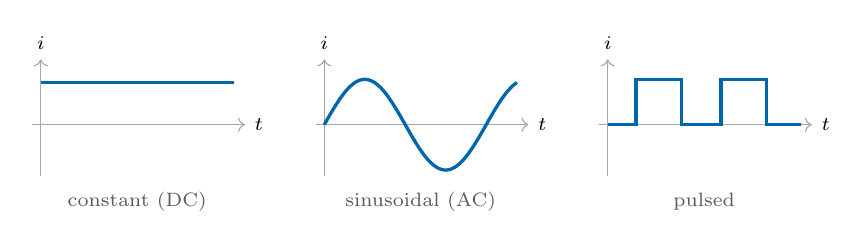
\begin{tikzpicture}[scale=0.72]
   \foreach \dx/\ttl in {0/{constant (DC)}, 5.0/{sinusoidal (AC)}, 10.0/{pulsed}}{
     \begin{scope}[xshift=\dx cm]
       \draw[->,gray!70] (-0.15,0) -- (3.6,0) node[right,font=\scriptsize,black] {$t$};
       \draw[->,gray!70] (0,-0.9) -- (0,1.15) node[above,font=\scriptsize,black] {$i$};
       \node[font=\scriptsize, text=metugray] at (1.7,-1.35) {\ttl};
     \end{scope}}
   \draw[ccur, very thick] (0,0.75) -- (3.4,0.75);
   \begin{scope}[xshift=5.0cm]
     \draw[ccur, very thick, domain=0:3.4, samples=120, smooth]
          plot (\x, {0.8*sin(deg(2.2*\x))});
   \end{scope}
   \begin{scope}[xshift=10.0cm]
     \draw[ccur, very thick] (0,0)--(0.5,0)--(0.5,0.8)--(1.3,0.8)--(1.3,0)
          --(2.0,0)--(2.0,0.8)--(2.8,0.8)--(2.8,0)--(3.4,0);
   \end{scope}
  \end{tikzpicture}
  \end{center}
  \vfill
  \begin{center}\small
    Only the first deserves the symbol $I$.
  \end{center}
\end{frame}

%--------------------------------------------------------------
\begin{frame}{Example: charging a phone}
  The last part of a charge cycle: the charge \emph{stored in the battery} approaches its
  full value, $q(t) = Q_f\left(1 - e^{-t/\tau}\right)$, with $Q_f = 3600\Cb$ and
  $\tau = 20$ min.
  \vspace{-0.2em}
  \begin{columns}[c,onlytextwidth]
    \column{0.57\textwidth}
      \begin{center}
      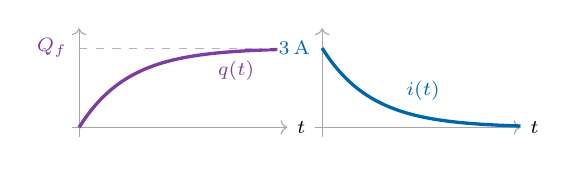
\begin{tikzpicture}[scale=0.63]
        % q(t)
        \draw[->,gray!70] (-0.15,0) -- (4.2,0) node[right,font=\scriptsize,black] {$t$};
        \draw[->,gray!70] (0,-0.2) -- (0,2.0);
        \draw[ccharge, very thick, domain=0:4.0, samples=120, smooth]
             plot (\x, {1.6*(1-exp(-\x))});
        \draw[ccharge!45, dashed] (0,1.6) -- (4.0,1.6);
        \node[ccharge, font=\scriptsize, right] at (2.6,1.15) {$\Qcol{q(t)}$};
        \node[ccharge, font=\scriptsize, left] at (-0.05,1.6) {$Q_f$};
        % i(t)
        \begin{scope}[xshift=4.9cm]
          \draw[->,gray!70] (-0.15,0) -- (4.0,0) node[right,font=\scriptsize,black] {$t$};
          \draw[->,gray!70] (0,-0.2) -- (0,2.0);
          \draw[ccur, very thick, domain=0:4.0, samples=120, smooth]
               plot (\x, {1.6*exp(-\x)});
          \node[ccur, font=\scriptsize, right] at (1.5,0.75) {$\Icol{i(t)}$};
          \node[ccur, font=\scriptsize, left] at (-0.05,1.6) {$3\A$};
        \end{scope}
      \end{tikzpicture}
      \end{center}
    \column{0.40\textwidth}
      \[ \Icol{i(t)} = \frac{dq}{dt} = \frac{Q_f}{\tau}\,e^{-t/\tau} \]
      \begin{itemize}
        \item $i(0) = 3600/1200 = 3\A$
        \item after $20$ min: $i = 3/e \approx 1.1\A$
        \item the fuller it gets, the slower it fills
      \end{itemize}
  \end{columns}
  \vfill
  \begin{center}\small
    \Qcol{Charge} is what accumulates; \Icol{current} is how fast it accumulates.
  \end{center}
\end{frame}

%==============================================================
\section{Voltage}
%--------------------------------------------------------------
\begin{frame}{\Vcol{Voltage}: why the charge moves}
  Charge does not move by itself. Pushing it through an element \alert{costs or releases
  energy} --- and that is what voltage measures.
  \vfill
  \begin{center}
  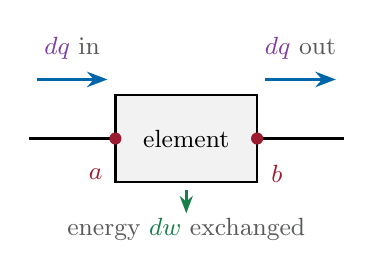
\begin{tikzpicture}[scale=1.0]
    \draw[thick] (0,0) -- (1.1,0); \draw[thick] (2.9,0) -- (4.0,0);
    \draw[thick, fill=gray!10] (1.1,-0.55) rectangle (2.9,0.55);
    \node[font=\small] at (2.0,0) {element};
    \node[font=\small, text=metured] at (0.85,-0.45) {$a$};
    \node[font=\small, text=metured] at (3.15,-0.45) {$b$};
    \fill[metured] (1.1,0) circle (2.2pt); \fill[metured] (2.9,0) circle (2.2pt);
    \draw[curarr] (0.1,0.75) -- (1.0,0.75);
    \node[font=\small, text=metugray] at (0.55,1.15) {\Qcol{$dq$} in};
    \draw[curarr] (3.0,0.75) -- (3.9,0.75);
    \node[font=\small, text=metugray] at (3.45,1.15) {\Qcol{$dq$} out};
    \node[font=\small, text=metugray] at (2.0,-1.15) {energy \Pcol{$dw$} exchanged};
    \draw[-{Stealth[length=2.2mm]}, cpow, very thick] (2.0,-0.65) -- (2.0,-0.95);
  \end{tikzpicture}
  \end{center}
  \vfill
  \begin{block}{Definition}
    \[ \Vcol{v_{ab}} \;=\; \frac{\Pcol{dw}}{\Qcol{dq}}
       \qquad\text{unit: \textbf{volt (V)}}, \quad 1\V = 1\J/\Cb \]
    the energy exchanged \emph{per unit of charge} carried from $a$ to $b$ through the
    element.
  \end{block}
\end{frame}

%--------------------------------------------------------------
\begin{frame}{What that definition does --- and does not --- say}
  \vfill
  \begin{itemize}\itemsep1.1em
    \item It is a \alert{ratio}. Twice the charge, twice the energy --- same $v_{ab}$.
          Voltage belongs to the \textbf{pair of points}, not to the charge.
    \item It is defined with \alert{nothing moving}. A $1.5\V$ battery on the shelf has
          $1.5\V$ across it at $i=0$ --- like a closed tap with pressure behind it.
    \item \alert{Order matters}: $v_{ab} = -v_{ba}$. There is no ``voltage at a point''
          until we fix a reference.
    \item The energy per charge depends on the two endpoints, \alert{not on the path}.
          That is what makes ``the voltage between $a$ and $b$'' mean anything --- and
          later it becomes KVL.
  \end{itemize}
  \vfill
\end{frame}

%--------------------------------------------------------------
\begin{frame}{Voltage is an electrical \alert{height}}
  \begin{columns}[c,onlytextwidth]
    \column{0.52\textwidth}
      \begin{center}
      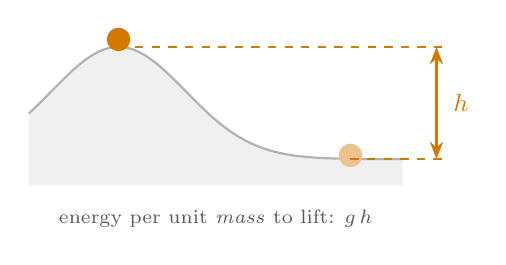
\begin{tikzpicture}[scale=0.95]
        \fill[gray!12] plot[domain=0:5, samples=100] (\x, {0.35+1.5*exp(-(\x-1.2)^2/1.6)})
              -- (5,0) -- (0,0) -- cycle;
        \draw[gray!60, thick] plot[domain=0:5, samples=100]
              (\x, {0.35+1.5*exp(-(\x-1.2)^2/1.6)});
        \node[circle, fill=cvolt, inner sep=3pt] at (1.2,1.95) {};
        \node[circle, fill=cvolt!45, inner sep=3pt] at (4.3,0.4) {};
        \draw[cvolt, thick, dashed] (1.2,1.85) -- (5.6,1.85);
        \draw[cvolt, thick, dashed] (4.3,0.35) -- (5.6,0.35);
        \draw[{Stealth[length=2.2mm]}-{Stealth[length=2.2mm]}, cvolt, very thick]
              (5.45,1.85) -- (5.45,0.35);
        \node[cvolt, font=\small, right] at (5.55,1.1) {$h$};
        \node[font=\scriptsize, text=metugray] at (2.5,-0.45)
             {energy per unit \emph{mass} to lift: $g\,h$};
      \end{tikzpicture}
      \end{center}
    \column{0.44\textwidth}
      \begin{itemize}
        \item Only the height \alert{difference} matters.
        \item ``Sea level'' is a \alert{choice} --- and changing it changes no physics.
        \item A heavier ball gains more energy, but energy \emph{per kilogram} is the
              same: that is why $g h$, like voltage, is a property of the two places.
      \end{itemize}
      \vspace{0.4em}
      {\small Voltage is the electrical version of this, with charge in place of mass.}
  \end{columns}
\end{frame}

%--------------------------------------------------------------
\begin{frame}{Charge is the \alert{amount}, voltage is the \alert{level}}
  \begin{columns}[c,onlytextwidth]
    \column{0.50\textwidth}
      \begin{center}
      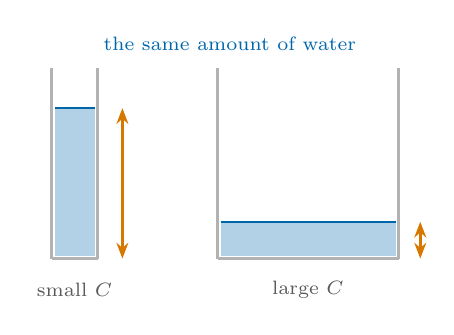
\begin{tikzpicture}[scale=0.78]
        \draw[gray!60, very thick] (0,0) -- (0,3.1);
        \draw[gray!60, very thick] (0.75,0) -- (0.75,3.1);
        \draw[gray!60, very thick] (0,0) -- (0.75,0);
        \fill[ccur!30] (0.05,0.05) rectangle (0.70,2.45);
        \draw[ccur, thick] (0.05,2.45) -- (0.70,2.45);
        \draw[{Stealth[length=2mm]}-{Stealth[length=2mm]}, cvolt, very thick] (1.15,0) -- (1.15,2.45);
        \node[font=\scriptsize, text=metugray] at (0.37,-0.5) {small $C$};
        \begin{scope}[xshift=2.7cm]
          \draw[gray!60, very thick] (0,0) -- (0,3.1);
          \draw[gray!60, very thick] (2.95,0) -- (2.95,3.1);
          \draw[gray!60, very thick] (0,0) -- (2.95,0);
          \fill[ccur!30] (0.05,0.05) rectangle (2.90,0.60);
          \draw[ccur, thick] (0.05,0.60) -- (2.90,0.60);
          \draw[{Stealth[length=2mm]}-{Stealth[length=2mm]}, cvolt, very thick] (3.3,0) -- (3.3,0.60);
          \node[font=\scriptsize, text=metugray] at (1.47,-0.5) {large $C$};
        \end{scope}
        \node[font=\scriptsize, text=ccur] at (2.9,3.5) {the same amount of water};
      \end{tikzpicture}
      \end{center}
    \column{0.46\textwidth}
      \[ q = C\,v \]
      \begin{itemize}
        \item \Qcol{charge} --- the amount poured in
        \item \Vcol{voltage} --- the level it reaches
        \item $C$ --- the cross-section of the container
      \end{itemize}
      \vspace{0.4em}
      {\small The \alert{shape of the circuit} plays the part of the shape of the tank.
       We define $C$ properly in Lecture~5.}
  \end{columns}
\end{frame}


%--------------------------------------------------------------
\begin{frame}{Reference polarity}
  Exactly as for current, we mark $+$ and $-$ \alert{before} we know the answer.
  \vfill
  \begin{center}
  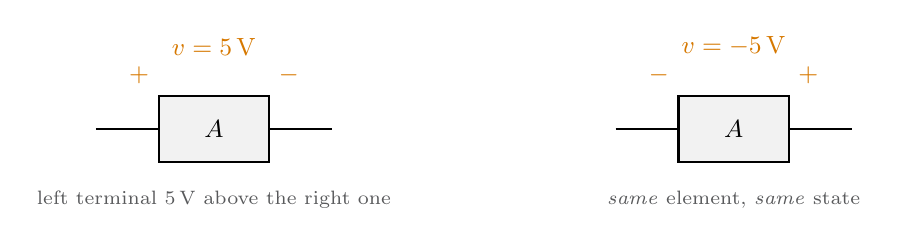
\begin{tikzpicture}[scale=1.0]
    \begin{scope}
      \draw[thick] (0,0) -- (0.8,0); \draw[thick] (2.2,0) -- (3.0,0);
      \draw[thick, fill=gray!10] (0.8,-0.42) rectangle (2.2,0.42);
      \node[font=\small] at (1.5,0) {$A$};
      \node[cvolt, font=\small] at (0.55,0.68) {$+$};
      \node[cvolt, font=\small] at (2.45,0.68) {$-$};
      \node[cvolt, font=\small] at (1.5,1.05) {$\Vcol{v = 5\V}$};
      \node[font=\scriptsize, text=metugray] at (1.5,-0.9) {left terminal $5\V$ above the right one};
    \end{scope}
    \begin{scope}[xshift=6.6cm]
      \draw[thick] (0,0) -- (0.8,0); \draw[thick] (2.2,0) -- (3.0,0);
      \draw[thick, fill=gray!10] (0.8,-0.42) rectangle (2.2,0.42);
      \node[font=\small] at (1.5,0) {$A$};
      \node[cvolt, font=\small] at (0.55,0.68) {$-$};
      \node[cvolt, font=\small] at (2.45,0.68) {$+$};
      \node[cvolt, font=\small] at (1.5,1.05) {$\Vcol{v = -5\V}$};
      \node[font=\scriptsize, text=metugray] at (1.5,-0.9) {\emph{same} element, \emph{same} state};
    \end{scope}
  \end{tikzpicture}
  \end{center}
  \vfill
  \begin{center}\small
    Same physical situation, two bookkeeping choices --- exactly like the current arrow.
  \end{center}
\end{frame}

%--------------------------------------------------------------
\begin{frame}{A first element: the \alert{resistor}}
  We have defined the variables. To talk about a circuit we also need an
  \emph{element} --- a rule tying $v$ and $i$ together. Here is the simplest one.
  \vfill
  \begin{columns}[c,onlytextwidth]
    \column{0.46\textwidth}
      \begin{block}{Ohm's law}
        \[ \Vcol{v} = R\,\Icol{i} \]
        \centering\small $R$ in ohms ($\Omega$), \quad $1\,\Omega = 1\V/\A$
      \end{block}
      \begin{center}
      \begin{circuitikz}[scale=0.9, transform shape]
        \draw (0,0) to[R, l_=$R$, v^=\mbox{\color{cvolt}$v$}, i>_=\mbox{\color{ccur}$i$}] (3,0);
      \end{circuitikz}
      \end{center}
    \column{0.50\textwidth}
      \begin{itemize}
        \item \textbf{Algebraic, no memory:} the current \emph{now} depends only on the
              voltage \emph{now} --- no derivatives, no history.
        \item \textbf{Geometry sets $R$:} for a uniform bar,
              \[ R = \rho\,\frac{L}{A} \]
              long and thin $\Rightarrow$ large $R$; short and fat $\Rightarrow$ small $R$.
              Exactly like a pipe.
      \end{itemize}
  \end{columns}
  \vfill
  \begin{center}\small\color{metugray}
    The full family of elements --- and the sign convention that goes with them ---
    comes in Lecture~2.
  \end{center}
\end{frame}

%--------------------------------------------------------------
\begin{frame}{The hydraulic analogy}
  \vfill
  \begin{center}
  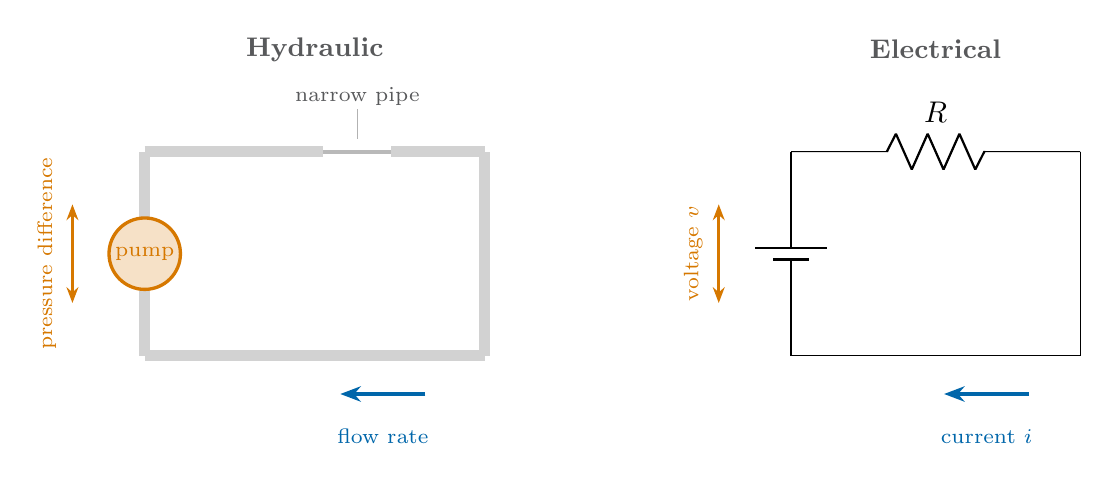
\begin{tikzpicture}[scale=1.08, transform shape]
    \node[font=\bfseries\small, text=metugray] at (2.0,3.6) {Hydraulic};
    \draw[line width=4pt, gray!35] (0,0) -- (0,2.4);
    \draw[line width=4pt, gray!35] (4,0) -- (4,2.4);
    \draw[line width=4pt, gray!35] (0,0) -- (4,0);
    \draw[line width=4pt, gray!35] (0,2.4) -- (2.1,2.4);
    \draw[line width=1.4pt, gray!55] (2.1,2.4) -- (2.9,2.4);
    \draw[line width=4pt, gray!35] (2.9,2.4) -- (4,2.4);
    \node[font=\scriptsize, text=metugray, align=center] at (2.5,3.05) {narrow pipe};
    \draw[gray!60] (2.5,2.9) -- (2.5,2.55);
    \fill[cvolt!22] (0,1.2) circle (0.42);
    \draw[cvolt, very thick] (0,1.2) circle (0.42);
    \node[font=\scriptsize, text=cvolt] at (0,1.2) {pump};
    \draw[acr] (-0.85,0.62) -- (-0.85,1.78);
    \node[font=\scriptsize, text=cvolt, rotate=90] at (-1.15,1.2) {pressure difference};
    \draw[curarr] (3.3,-0.45) -- (2.3,-0.45);
    \node[font=\scriptsize, text=ccur] at (2.8,-0.95) {flow rate};
    \begin{scope}[xshift=7.6cm]
      \node[font=\bfseries\small, text=metugray] at (1.7,3.6) {Electrical};
      \draw (0,0) to[battery1, invert] (0,2.4);
      \draw[acr] (-0.85,0.62) -- (-0.85,1.78);
      \node[font=\scriptsize, text=cvolt, rotate=90] at (-1.15,1.2) {voltage $v$};
      \draw (0,2.4) to[R, l={$R$}] (3.4,2.4);
      \draw (3.4,2.4) -- (3.4,0) -- (0,0);
      \draw[curarr] (2.8,-0.45) -- (1.8,-0.45);
      \node[font=\scriptsize, text=ccur] at (2.3,-0.95) {current $i$};
    \end{scope}
  \end{tikzpicture}
  \end{center}
  \vfill
\end{frame}

%--------------------------------------------------------------
\begin{frame}{The dictionary}
  \vfill
  \begin{center}
  \renewcommand{\arraystretch}{1.35}
  \begin{tabular}{r c l}
    \toprule
    \textbf{Hydraulic} & & \textbf{Electrical}\\
    \midrule
    pressure difference  & $\leftrightarrow$ & \Vcol{voltage $v$}\\
    volumetric flow rate & $\leftrightarrow$ & \Icol{current $i$}\\
    pipe restriction     & $\leftrightarrow$ & resistance $R$\\
    pump                 & $\leftrightarrow$ & voltage source\\
    \bottomrule
  \end{tabular}
  \end{center}
  \vfill
  \begin{center}\small\color{metugray}
    Useful for intuition, not for proofs --- water is incompressible, charge is not.
  \end{center}
  \vfill
\end{frame}

%==============================================================
\section{Ground}
%--------------------------------------------------------------
\begin{frame}{Ground: the node we \alert{choose} to call zero}
  \begin{columns}[T,onlytextwidth]
    \column{0.46\textwidth}
      \begin{block}{Reference node}
        Only differences matter, so we are free to declare one node to be $0\V$. Then
        \[
          v_{ab} = v_a - v_b .
        \]
      \end{block}
      \vspace{0.3em}
      {\small Move the reference and \emph{every} node voltage shifts by the same
       constant. No two-point voltage, current or power changes.}
    \column{0.50\textwidth}
      \begin{center}
      \begin{circuitikz}[scale=0.8, transform shape]
        \draw (0,0) to[battery1, invert, l={$12\V$}] (0,2.4);
        \draw (0,2.4) -- (1.2,2.4);
        \draw (1.2,2.4) to[R, l_=$R_1$] (3.4,2.4);
        \draw (3.4,2.4) to[R, l=$R_2$] (3.4,0);
        \draw (3.4,0) -- (0,0);
        \draw (0,0) node[ground]{};
        \fill[cvolt] (1.2,2.4) circle (2.4pt);
        \fill[cvolt] (3.4,2.4) circle (2.4pt);
        \node[font=\small, text=cvolt, above] at (1.2,2.5) {$a$};
        \node[font=\small, text=cvolt, above] at (3.4,2.55) {$b$};
      \end{circuitikz}
      \end{center}
  \end{columns}
  \vfill
  {\footnotesize\color{metugray} Pick the node that the most elements touch --- your
   equations get shorter.}
\end{frame}

%--------------------------------------------------------------
\begin{frame}{Three different things are called ``ground''}
  \begin{columns}[T,onlytextwidth]
    \column{0.31\textwidth}
      \begin{block}{Earth ground}
        \small A physical connection to the planet. Safety.
      \end{block}
    \column{0.31\textwidth}
      \begin{block}{Chassis ground}
        \small The metal enclosure of the instrument.
      \end{block}
    \column{0.31\textwidth}
      \begin{block}{Signal ground}
        \small The analysis reference. \alert{This is ours.}
      \end{block}
  \end{columns}
  \vfill
  \begin{center}
    In EE201 we mean the third one.\\[3pt]
    {\small In the laboratory, confusing them is how you blow a fuse.}
  \end{center}
\end{frame}

%==============================================================
\section{Power}
%--------------------------------------------------------------
\begin{frame}{\Pcol{Power} falls out of the definitions}
  \vfill
  \[
    \Pcol{p(t)} = \frac{dw}{dt}
                = \underbrace{\frac{dw}{dq}}_{\Vcol{v(t)}}\cdot
                  \underbrace{\frac{dq}{dt}}_{\Icol{i(t)}}
                = \Vcol{v(t)}\,\Icol{i(t)}
  \]
  \vfill
  \begin{columns}[T,onlytextwidth]
    \column{0.48\textwidth}
      \begin{block}{Power}
        unit \textbf{watt (W)}, $1\W = 1\J/\s$
      \end{block}
    \column{0.48\textwidth}
      \begin{block}{Energy}
        \[ w = \int_{t_0}^{t} v(\tau)i(\tau)\,d\tau \]
      \end{block}
  \end{columns}
  \vfill
  \begin{center}\small
    $p = vi$ was \alert{not postulated} --- it is a consequence of defining $v$ as energy
    per charge and $i$ as charge per time.
  \end{center}
\end{frame}

%--------------------------------------------------------------
\begin{frame}{Power that changes in time}
  A resistive element with $v(t) = 10\cos\omega t\V$ and $i(t) = 2\cos\omega t\A$:
  \[
    p(t) = v i = 20\cos^{2}\omega t = 10\left(1 + \cos 2\omega t\right)\W
  \]
  \vfill
  \begin{center}
  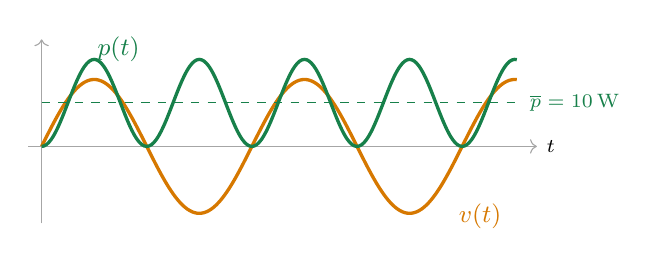
\begin{tikzpicture}[scale=0.85]
    \draw[->,gray!70] (-0.2,0) -- (7.4,0) node[right,font=\scriptsize,black] {$t$};
    \draw[->,gray!70] (0,-1.15) -- (0,1.6);
    \draw[cvolt, very thick, domain=0:7.1, samples=200, smooth]
         plot (\x, {1.0*sin(deg(2*\x))});
    \draw[cpow, very thick, domain=0:7.1, samples=200, smooth]
         plot (\x, {1.3*sin(deg(2*\x))*sin(deg(2*\x))});
    \draw[cpow, dashed] (0,0.65) -- (7.1,0.65);
    \node[cpow, font=\scriptsize, right] at (7.15,0.65) {$\overline{p} = 10\W$};
    \node[cpow, font=\small] at (1.15,1.45) {$\Pcol{p(t)}$};
    \node[cvolt, font=\small] at (6.55,-1.05) {$\Vcol{v(t)}$};
  \end{tikzpicture}
  \end{center}
  \vfill
  \begin{itemize}
    \item $p(t) \ge 0$: a resistor never gives energy back.
    \item The power ripples at \alert{twice} the frequency, around $\overline{p} = 10\W$.
  \end{itemize}
\end{frame}

%==============================================================
\section{Passive sign convention}
%--------------------------------------------------------------
\begin{frame}{The passive sign convention}
  \begin{block}{PSC}
    Draw the current arrow so that it \alert{enters the $+$ terminal}. Then
    \[ p = vi = \text{power \emph{absorbed} by the element}. \]
    $p > 0$: the element absorbs. \qquad $p < 0$: it delivers.
  \end{block}
  \begin{center}\small\color{metugray}
    Given a picture that does not obey the PSC: flip one reference, change that
    variable's sign, and use $p = vi$ as always.
  \end{center}
  \vfill
  \begin{center}
  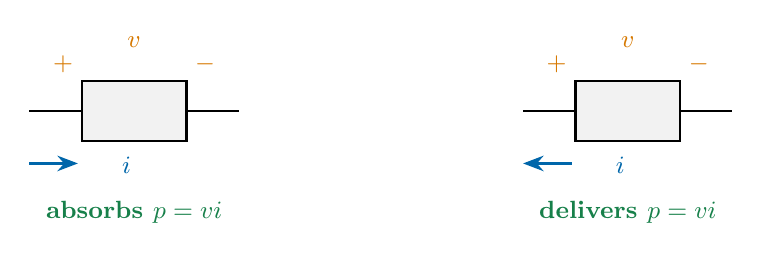
\begin{tikzpicture}[scale=0.95]
    \begin{scope}
      \draw[thick] (0,0) -- (0.7,0); \draw[thick] (2.1,0) -- (2.8,0);
      \draw[thick, fill=gray!10] (0.7,-0.4) rectangle (2.1,0.4);
      \node[cvolt, font=\small] at (0.45,0.62) {$+$};
      \node[cvolt, font=\small] at (2.35,0.62) {$-$};
      \node[cvolt, font=\small] at (1.4,0.92) {$\Vcol{v}$};
      \draw[curarr] (0.0,-0.7) -- (0.65,-0.7);
      \node[ccur, font=\small] at (1.3,-0.72) {$\Icol{i}$};
      \node[font=\small\bfseries, text=cpow] at (1.4,-1.35) {absorbs $p = vi$};
    \end{scope}
    \begin{scope}[xshift=6.6cm]
      \draw[thick] (0,0) -- (0.7,0); \draw[thick] (2.1,0) -- (2.8,0);
      \draw[thick, fill=gray!10] (0.7,-0.4) rectangle (2.1,0.4);
      \node[cvolt, font=\small] at (0.45,0.62) {$+$};
      \node[cvolt, font=\small] at (2.35,0.62) {$-$};
      \node[cvolt, font=\small] at (1.4,0.92) {$\Vcol{v}$};
      \draw[curarr] (0.65,-0.7) -- (0.0,-0.7);
      \node[ccur, font=\small] at (1.3,-0.72) {$\Icol{i}$};
      \node[font=\small\bfseries, text=cpow] at (1.4,-1.35) {delivers $p = vi$};
    \end{scope}
  \end{tikzpicture}
  \end{center}
\end{frame}

%--------------------------------------------------------------
\begin{frame}{Example: a power balance}
  \begin{columns}[T,onlytextwidth]
    \column{0.46\textwidth}
      \begin{center}
      \begin{circuitikz}[scale=0.85, transform shape]
        \draw (0,0) to[battery1, invert, l={$12\,$V}] (0,2.6);
        \node[font=\small, text=cvolt] at (-0.33,2.05) {$+$};
        \node[font=\small, text=cvolt] at (-0.33,0.55) {$-$};
        \draw (0,2.6) to[short, i>^={\color{ccur}$2\,$A}] (1.1,2.6);
        \draw (1.1,2.6) to[R, l_={$R_1$}, v^={\color{cvolt}$8\,$V}] (3.9,2.6);
        \draw (3.9,2.6) to[R, l={$R_2$}, v_={\color{cvolt}$4\,$V}] (3.9,0);
        \draw (3.9,0) -- (0,0);
      \end{circuitikz}
      \end{center}
    \column{0.50\textwidth}
      \begin{align*}
        p_{R_1} &= 8 \times 2 = +16\W\\
        p_{R_2} &= 4 \times 2 = +8\W\\
        p_{\text{src}} &= 12 \times (-2) = -24\W
      \end{align*}
      \vspace{-0.4em}
      \begin{center}
        $16 + 8 - 24 = 0$ \checkmark
      \end{center}
      {\small The source current \emph{leaves} its $+$ terminal --- hence $-2\A$.}
  \end{columns}
  \vfill
  \begin{center}\small
    In \emph{any} circuit, at \emph{every} instant, $\sum_k p_k(t) = 0$. If the powers in
    your solution do not cancel, your solution is wrong --- \alert{a free check, every time}.
  \end{center}
\end{frame}

%==============================================================
\section{Lumped circuits}
%--------------------------------------------------------------
\begin{frame}{What exactly is a circuit?}
  \vfill
  \begin{center}
    Elements interconnected so that charge can flow along \alert{closed paths}.\\[2pt]
    Everything in EE201 also assumes the circuit is \alert{lumped}:
  \end{center}
  \vfill
  \begin{block}{Three things we assume}
    \begin{enumerate}\itemsep0.55em
      \item \textbf{Nothing piles up.} Current out $=$ current in, at every instant.
            {\footnotesize Charge may \emph{separate} inside --- a capacitor does exactly
             that --- but the element as a whole never gains charge.}
      \item \textbf{Nothing leaks out.} No changing magnetic field through your loops:
            they are neither antennas nor transformers.
      \item \textbf{Nothing is late.} The circuit is much smaller than the wavelength,
            $d \ll \lambda = c/f$.
    \end{enumerate}
  \end{block}
  \vfill
  \begin{center}\footnotesize\color{metugray}
    $50$ Hz: $\lambda = 6000$ km --- any board is lumped. \qquad
    $2.4$ GHz: $\lambda = 12.5$ cm --- a $3$ cm track is not.
  \end{center}
  \vfill
\end{frame}

%--------------------------------------------------------------
\begin{frame}{Nothing is late: a circuit much smaller than $\lambda$}
  \begin{center}
  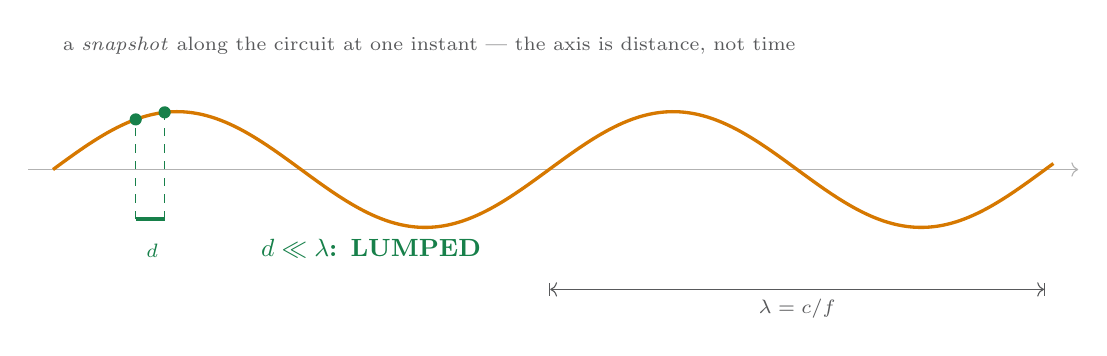
\begin{tikzpicture}[x=1.05cm,y=1.05cm]
    \draw[->,gray!60] (-0.3,0) -- (12.4,0);
    \draw[cvolt, very thick, domain=0:12.1, samples=300, smooth] plot (\x, {0.7*sin(60*\x)});
    \draw[metugray,|<->|] (6,-1.45) -- (12,-1.45) node[midway,below,font=\scriptsize] {$\lambda = c/f$};
    \node[font=\scriptsize, text=metugray, anchor=west] at (0,1.5)
         {a \emph{snapshot} along the circuit at one instant --- the axis is distance, not time};
    \fill[cpow] (1.0,{0.7*sin(60*1.0)}) circle (2.2pt);
    \fill[cpow] (1.35,{0.7*sin(60*1.35)}) circle (2.2pt);
    \draw[cpow,dashed,thin] (1.0,-0.6) -- (1.0,{0.7*sin(60*1.0)});
    \draw[cpow,dashed,thin] (1.35,-0.6) -- (1.35,{0.7*sin(60*1.35)});
    \draw[cpow, very thick] (1.0,-0.6) -- (1.35,-0.6);
    \node[font=\scriptsize, text=cpow, anchor=north] at (1.2,-0.78) {$d$};
    \node[font=\small\bfseries, text=cpow, anchor=west] at (2.4,-0.95) {$d \ll \lambda$: LUMPED};
  \end{tikzpicture}
  \end{center}
  \vfill
  \begin{center}
  Both ends sit at practically the same point of the wave, so every point of the circuit
  reads \alert{the same number} at any instant ---\\ ``the voltage of a node'' means
  something.
  \end{center}
  \vfill
\end{frame}

%--------------------------------------------------------------
\begin{frame}{\dots and one that is not}
  \begin{center}
  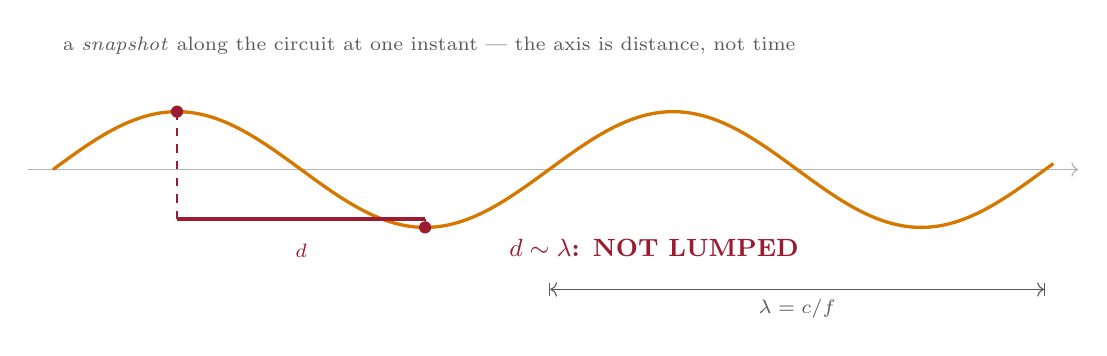
\begin{tikzpicture}[x=1.05cm,y=1.05cm]
    \draw[->,gray!60] (-0.3,0) -- (12.4,0);
    \draw[cvolt, very thick, domain=0:12.1, samples=300, smooth] plot (\x, {0.7*sin(60*\x)});
    \draw[metugray,|<->|] (6,-1.45) -- (12,-1.45) node[midway,below,font=\scriptsize] {$\lambda = c/f$};
    \node[font=\scriptsize, text=metugray, anchor=west] at (0,1.5)
         {a \emph{snapshot} along the circuit at one instant --- the axis is distance, not time};
    \fill[metured] (1.5,0.7) circle (2.2pt);
    \fill[metured] (4.5,-0.7) circle (2.2pt);
    \draw[metured,dashed,thin] (1.5,-0.6) -- (1.5,0.7);
    \draw[metured,dashed,thin] (4.5,-0.6) -- (4.5,-0.7);
    \draw[metured, very thick] (1.5,-0.6) -- (4.5,-0.6);
    \node[font=\scriptsize, text=metured, anchor=north] at (3.0,-0.78) {$d$};
    \node[font=\small\bfseries, text=metured, anchor=west] at (5.4,-0.95) {$d \sim \lambda$: NOT LUMPED};
  \end{tikzpicture}
  \end{center}
  \vfill
  \begin{center}
  One end is at the crest, the other at the trough: \alert{different values at the same
  moment}.\\ There is no single number to call the node voltage, and circuit theory no
  longer applies.
  \end{center}
  \vfill
\end{frame}

%--------------------------------------------------------------
%==============================================================
\section{Topology}
%--------------------------------------------------------------
\begin{frame}{Terminals, nodes, branches, loops}
  \begin{columns}[T,onlytextwidth]
    \column{0.52\textwidth}
      \begin{itemize}
        \item \textbf{Terminal} --- a point where an element connects. R, L, C: two.
              Transistor: three.
        \item \textbf{Node} --- a connection point. Everything joined by ideal wire is
              \alert{one} node, however long the wire.
        \item \textbf{Branch} --- one element between two nodes.
        \item \textbf{Loop} --- a closed path through no node twice.
      \end{itemize}
      \vspace{0.4em}
      \[ \#\text{branches} = \#\text{loops} + \#\text{nodes} - 1 \]
    \column{0.44\textwidth}
      \begin{center}
      \begin{circuitikz}[scale=0.75, transform shape]
        \draw (0,0) to[battery1, invert, l={$V_s$}] (0,2.4);
        \draw (0,2.4) -- (1.0,2.4);
        \draw (1.0,2.4) to[R, l_=$R_1$] (3.4,2.4);
        \draw (3.4,2.4) to[R, l=$R_2$] (3.4,0);
        \draw (3.4,2.4) -- (5.0,2.4);
        \draw (5.0,2.4) to[R, l=$R_3$] (5.0,0);
        \draw (5.0,0) -- (0,0);
        \draw (0,0) node[ground]{};
        \foreach \p in {(1.0,2.4),(3.4,2.4),(5.0,2.4)}{\fill[metured] \p circle (2.6pt);}
        \fill[metured] (0,0) circle (2.6pt);
        \node[font=\small, text=metured, above] at (0.7,2.5) {$n_1$};
        \node[font=\small, text=metured, above] at (3.4,2.6) {$n_2$};
        \node[font=\small, text=metured, below] at (1.7,-0.1) {$n_3$};
      \end{circuitikz}
      \end{center}
      \begin{center}\small $4 = 2 + 3 - 1$\end{center}
  \end{columns}
\end{frame}

%--------------------------------------------------------------
\begin{frame}{The same circuit, drawn twice}
  \begin{columns}[c,onlytextwidth]
    \column{0.50\textwidth}
      \begin{center}
      \begin{circuitikz}[scale=0.62, transform shape]
        \draw (0,0) to[battery1, invert, l={$V_s$}] (0,2.8);
        \draw (0,2.8) -- (1.6,2.8);
        \draw (1.6,2.8) to[R, l_={$R_1$}] (1.6,1.0);
        \draw (3.6,2.8) to[R, l={$R_2$}] (3.6,1.0);
        \draw (1.6,2.8) -- (3.6,2.8);
        \draw (1.6,1.0) -- (3.6,1.0);
        \draw (1.6,1.0) -- (1.6,0.5);
        \draw (3.6,1.0) -- (3.6,0.5);
        \draw (1.6,0.5) -- (5.8,0.5);
        \draw (5.8,0.5) to[R, l={$R_3$}] (5.8,2.8);
        \draw (5.8,2.8) -- (6.9,2.8) -- (6.9,0) -- (0,0);
        \draw (0,0) node[ground]{};
      \end{circuitikz}\\[2pt]
      {\scriptsize\color{metugray} drawing (a)}
      \end{center}
    \column{0.46\textwidth}
      \begin{center}
      \begin{circuitikz}[scale=0.72, transform shape]
        \draw (0,0) to[battery1, invert, l={$V_s$}] (0,2.6);
        \draw (0,2.6) -- (1.2,2.6);
        \draw (1.2,2.6) to[R, l_={$R_1$}] (3.0,2.6);
        \draw (1.2,1.5) to[R, l_={$R_2$}] (3.0,1.5);
        \draw (1.2,2.6) -- (1.2,1.5);
        \draw (3.0,2.6) -- (3.0,1.5);
        \draw (3.0,2.05) -- (4.0,2.05);
        \draw (4.0,2.05) to[R, l={$R_3$}] (4.0,0);
        \draw (4.0,0) -- (0,0);
        \draw (0,0) node[ground]{};
      \end{circuitikz}\\[2pt]
      {\scriptsize\color{metugray} drawing (b)}
      \end{center}
  \end{columns}
  \vfill
  \begin{center}
    Same circuit. \alert{Drawing is not topology.}\\
    {\small When a problem looks impossible, redraw it so that everything joined to the
     same node sits together --- the series and parallel connections then show themselves.}
  \end{center}
\end{frame}

%==============================================================
%--------------------------------------------------------------
\begin{frame}{Summary}
  \begin{center}
  \small
  \begin{tabular}{l c l l}
    \toprule
    \textbf{Quantity} & \textbf{Symbol} & \textbf{Definition} & \textbf{Unit}\\
    \midrule
    charge  & \Qcol{$q$} & ---              & C\\
    current & \Icol{$i$} & $i = dq/dt$      & A $=$ C/s\\
    voltage & \Vcol{$v$} & $v = dw/dq$      & V $=$ J/C\\
    power   & \Pcol{$p$} & $p = vi$         & W $=$ J/s\\
    energy  & \Pcol{$w$} & $w = \int p\,dt$ & J\\
    \bottomrule
  \end{tabular}
  \end{center}
  \vfill
  \begin{itemize}
    \item References (arrow, polarity) are \alert{choices}; signs carry the physics.
    \item PSC: current into $+$ $\Rightarrow$ $p = vi$ is absorbed, and $\sum_k p_k = 0$.
    \item Across vs through. Ground is a choice.
    \item Lumped $\Rightarrow$ ODEs. That is what makes this course possible.
  \end{itemize}
\end{frame}

%--------------------------------------------------------------
\begin{frame}{Next lecture}
  \begin{block}{Interconnection laws}
    Kirchhoff's current law (conservation of charge) and Kirchhoff's voltage law
    (conservation of energy), then the branch relations of the basic elements.
  \end{block}
  \vfill
  \begin{center}
    \Large\color{metured}\textbf{Questions?}\\[6pt]
    \normalsize\normalcolor
    Notes for this lecture: see the course repository.
  \end{center}
\end{frame}

\end{document}
